%\documentclass{article}
%\usepackage{graphicx}
%\usepackage{caption}
%\usepackage{subcaption}
%
%\begin{document}
\begin{figure}[!tbp]
  \centering
	\fbox{  
	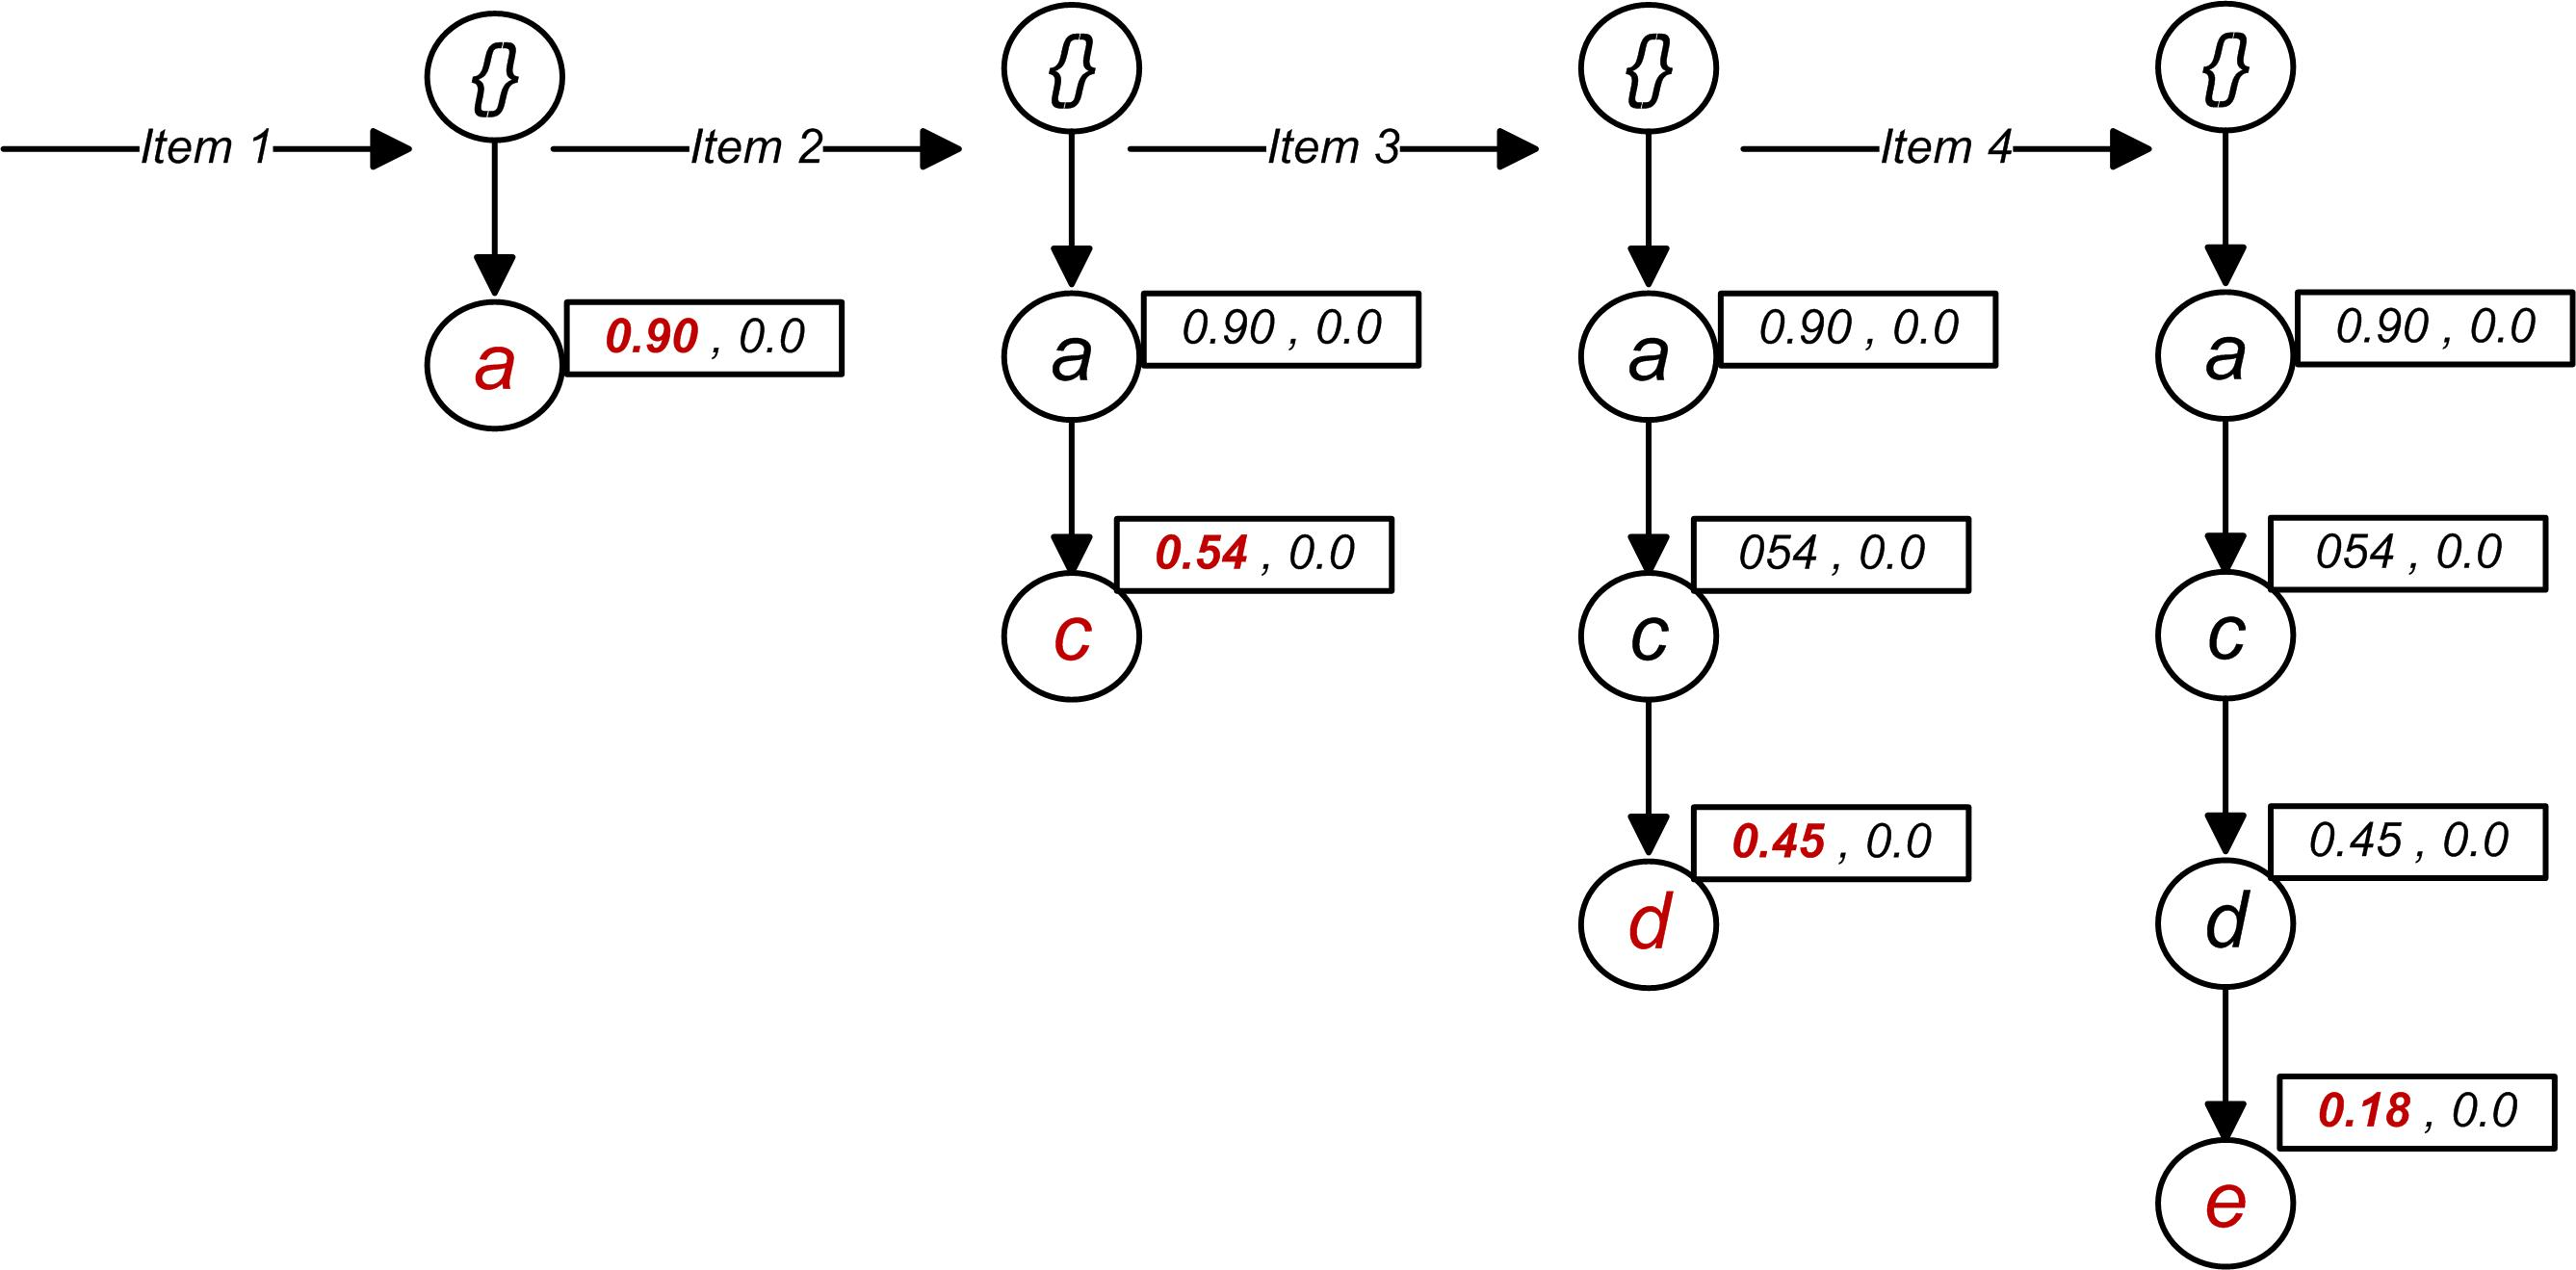
\includegraphics[width=.8\textwidth,height=5cm]{../images/sim_01.jpg}  
	}
	\caption{Inserting \emph{T-1} into \emph{US-tree}}
\end{figure}
\begin{frame}

\begin{figure}[!tbp]
  \centering
	\fbox{  
	 	\begin{subfigure}[b]{0.40\textwidth}
	 	\centering
	    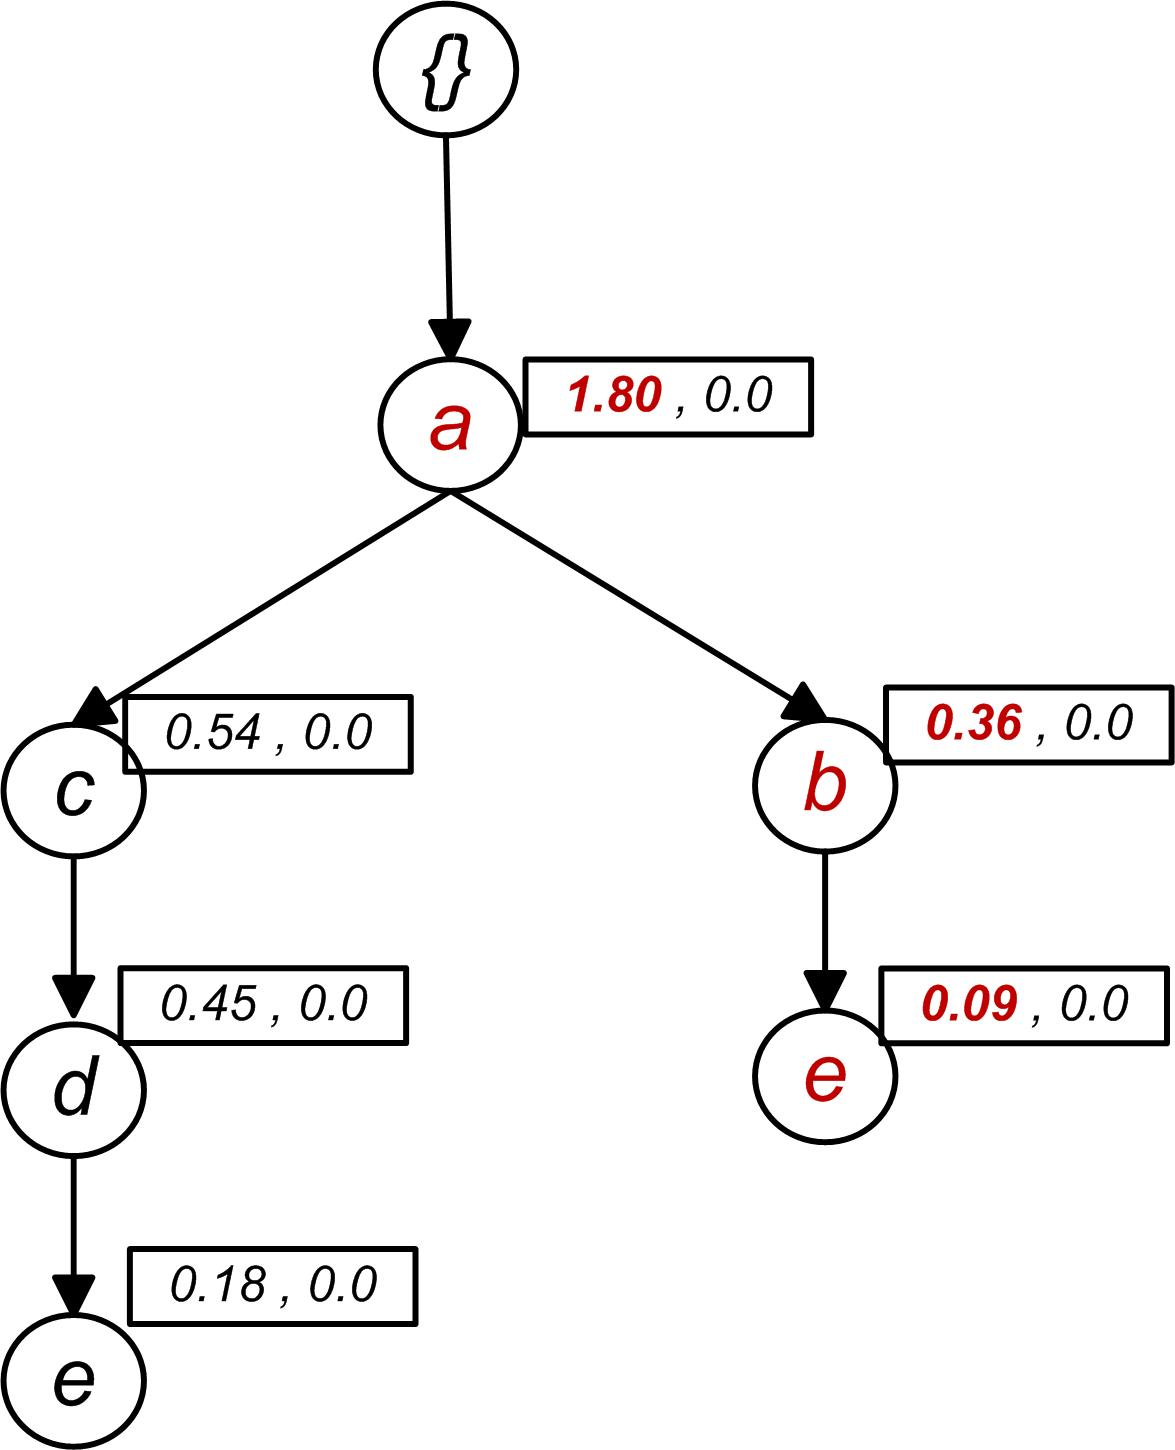
\includegraphics[width=.8\textwidth,height=4cm]{../images/sim_02.jpg}
	    \caption{T2}
		\end{subfigure}
	  
	 	\begin{subfigure}[b]{0.40\textwidth}
	 	\centering
	    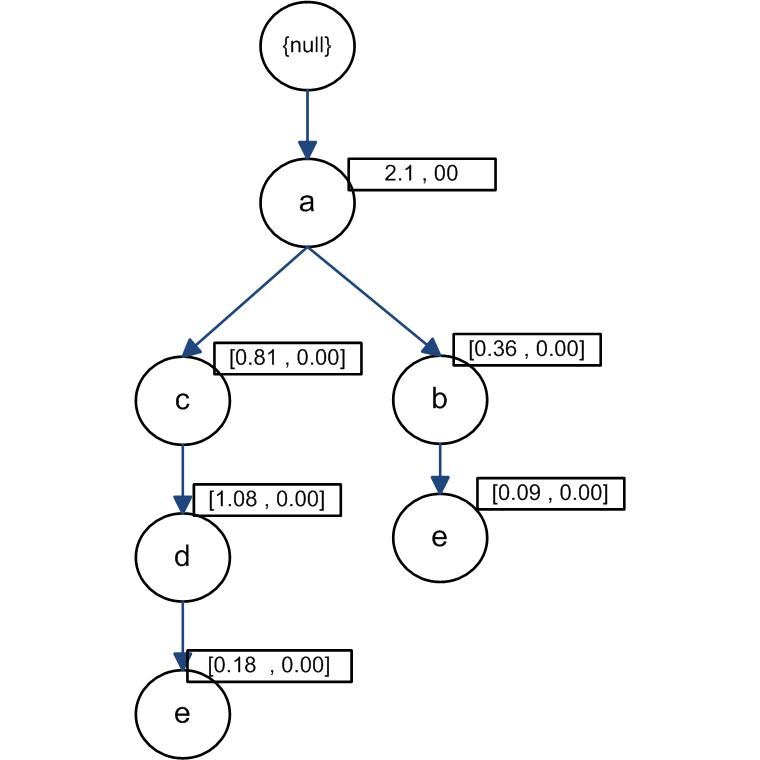
\includegraphics[width=.8\textwidth,height=4cm]{../images/sim_03.jpg}
	    \caption{T3}
		\end{subfigure}
	}
 \caption{Inserting \emph{T-2} and \emph{T-3} in \emph{US-tree}}
\end{figure}
\end{frame}
\begin{frame}

\begin{figure}[!tbp]
  \centering
	\fbox{  
	 	\begin{subfigure}[b]{0.22\textwidth}
	 	\centering
	    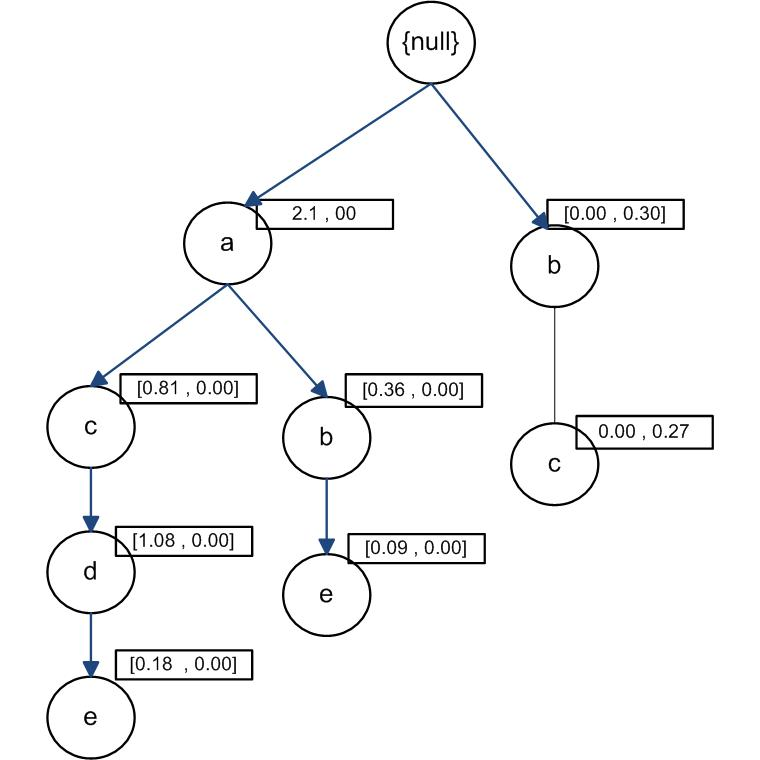
\includegraphics[width=\textwidth,height=4.0cm]{../images/sim_04.jpg}
	    \caption{T4}
		\end{subfigure}
	 
	 	\begin{subfigure}[b]{0.27\textwidth}
	 	\centering
	    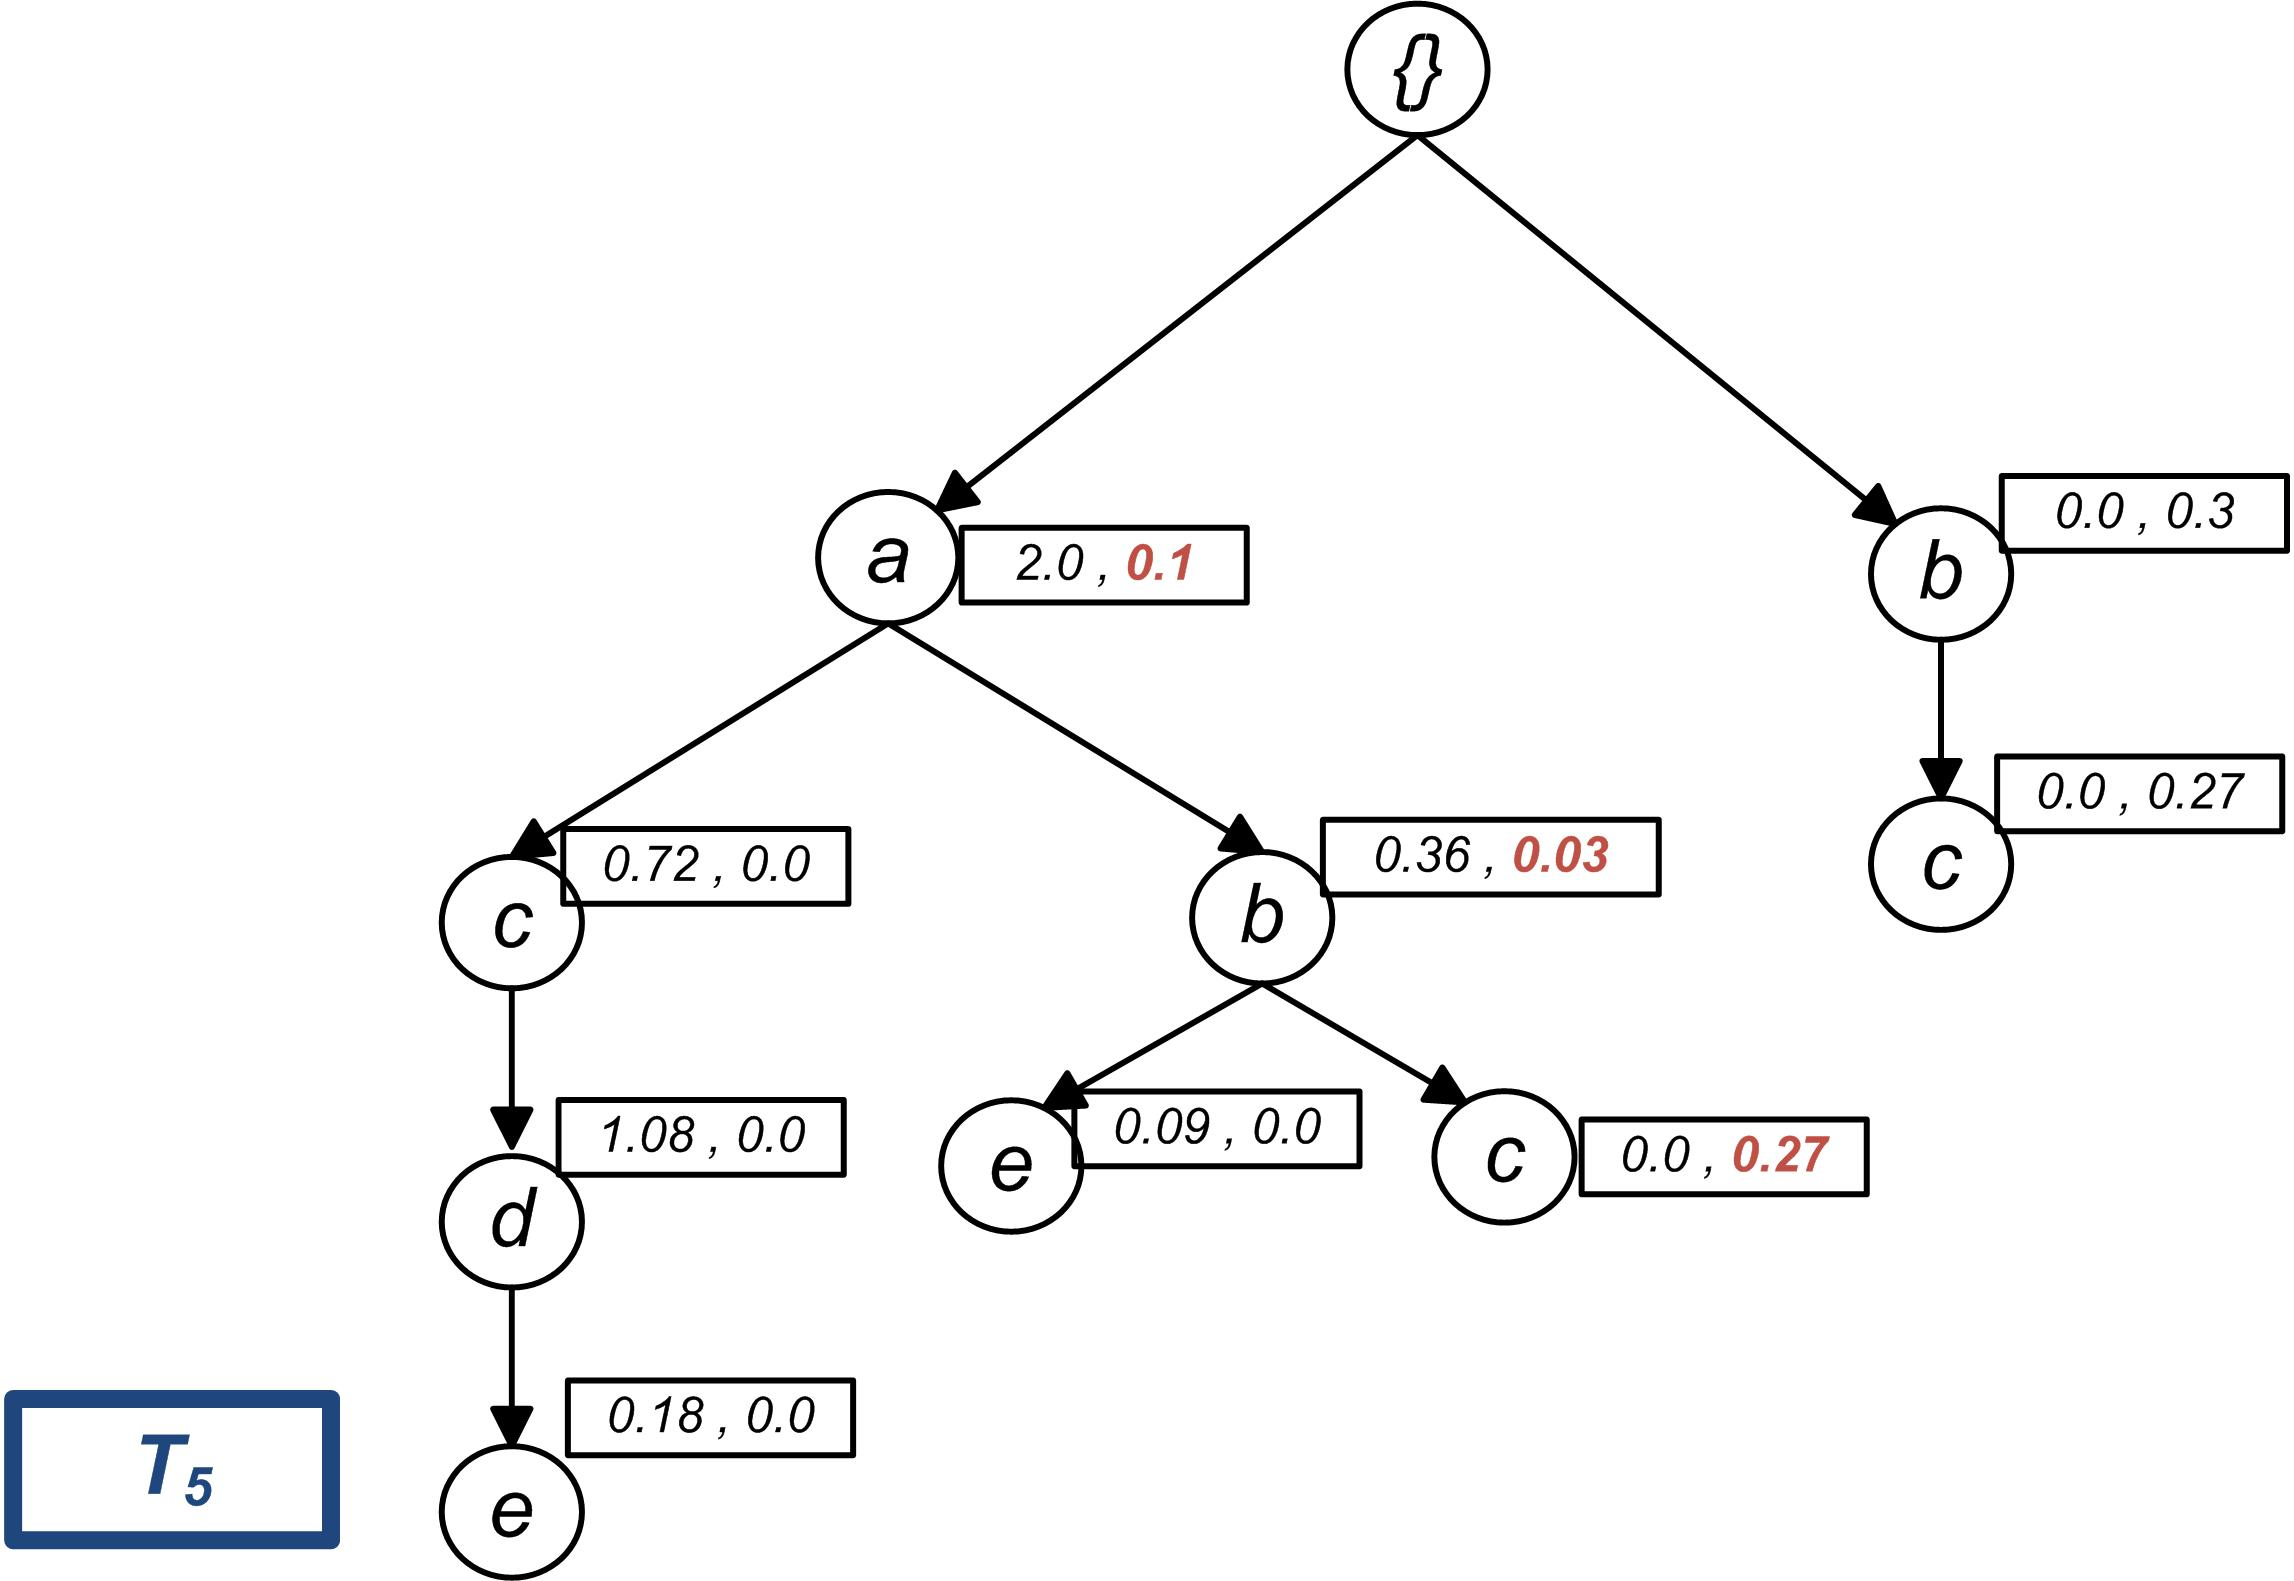
\includegraphics[width=\textwidth,height=4.0cm]{../images/sim_05.jpg}
	    \caption{T6}
		\end{subfigure}
	  
	 	\begin{subfigure}[b]{0.31\textwidth}
	 	\centering
	    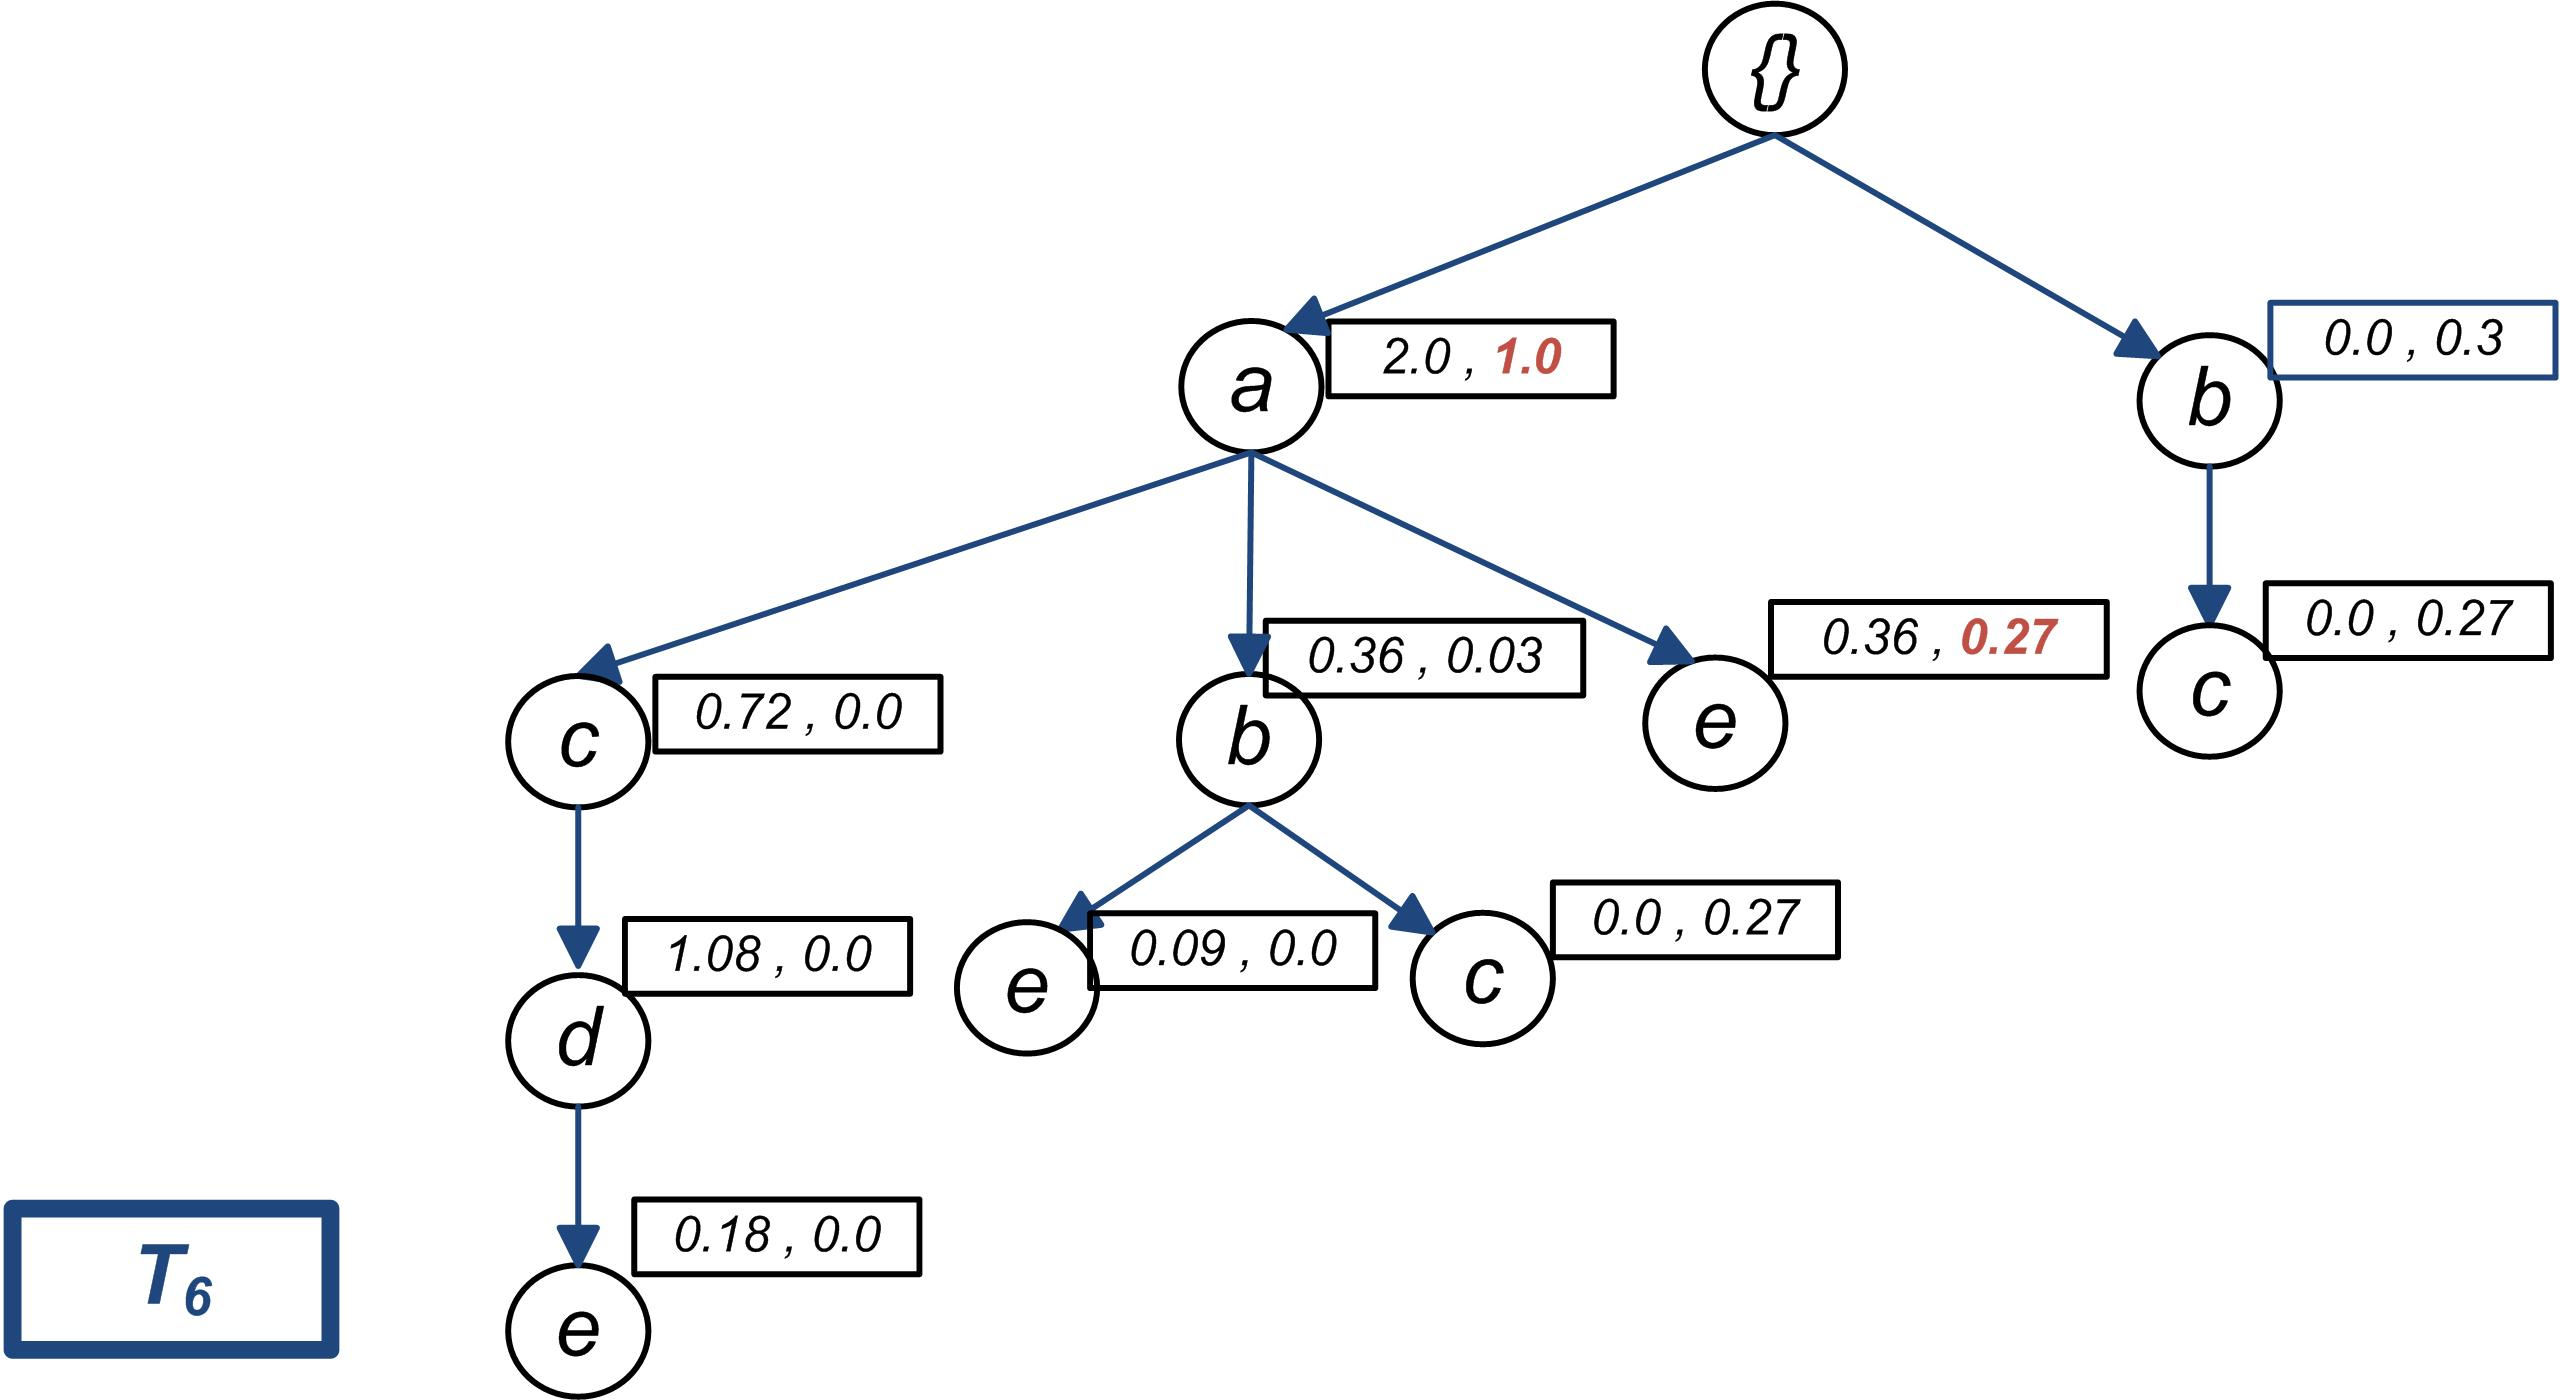
\includegraphics[width=\textwidth,height=3.0cm]{../images/sim_06.jpg}
	    \caption{T6}
		\end{subfigure}
	}
 \caption{Inserting \emph{T-4},\emph{T-5} and \emph{T-6} in \emph{US-tree}}
\end{figure}
\end{frame}
%\end{document}